\documentclass[conference,12pt]{IEEEtran}

\usepackage[tight,footnotesize]{subfigure}

\ifCLASSINFOpdf
  \usepackage[pdftex]{graphicx}
  \graphicspath{{./images/}}
\else
\fi

\usepackage[cmex10]{amsmath}


\hyphenation{op-tical net-works semi-conduc-tor}

\begin{document}
	
\title{System Design Project
	\\Group 12 - Robot Unicorn Defenders
	\\Group report 2}

\author{
\IEEEauthorblockN{Jonas Galdikas, Calum Jackson, Daria Kuznetsova, 
Roberto Bezoari,\\ Marc Howarth, Juozas Kaziukenas, Biser Hong, 
Aleksandar Krastev, Behzad Tabibian}
\IEEEauthorblockA{University of Edinburgh}
}
	
\maketitle
\numberwithin{equation}{section}
\IEEEpeerreviewmaketitle

\pagebreak
	
\section{Introduction}
\vspace{-2 mm}
In the second phase of the System Design Project, we broadened our goals from simply focusing on accomplishing the milestone to also planning for the future. This was reflected in the work we have been doing, which includes:
\begin{itemize}
\item Investigating and implementing planning and path-finding algorithms  
\item Planning basic gaming strategy
\item Implementing a simulator for testing strategy and movement
\end{itemize}
\vspace{-2 mm}
\section{Team Organisation}
\vspace{-2 mm}
After the completion of the first milestone, our groups were reorganised in view of our new goals. We wanted to put more focus on programming robot movement, and strategy for the future, so a member of the Vision team was reassigned to Movement and Behaviour. This was also beneficial in aiding the integration of the previously independent Vision system with the Client/Server system controlling the robots movement. To facilitate better group coordination and integration, a Team Manager was elected, to oversee whole-group interaction. Also design of Team logo is now finalized. The original design started by Roberto and completed by Biser, Figure \ref{fig:logo}.
\vspace{-2 mm}
\section{Construction}	
\vspace{-2 mm}
This period of robot construction consisted largely of tuning and adapting the existing design, and troubleshooting a number of problems. Our main goal was to ensure reliable movement in a straight line from the robot, as this was a problem with the robot used for the first milestone.

While the existing design was an acceptable base to work with, it had a number of problems, predominantly with the wheels. The four wheeled design was significantly flawed, as the two back caster wheels would swivel freely, frequently sending the robot off a straight course. In attempt to fix this problem, we experimented with a large number of different tyres and wheel arrangements. We also acquired two large ball-bearings to use instead of caster wheels at the rear or the robot. These proved much more reliable than casters, as they did not affect the robot's steering in any way.

The most successful wheel arrangement proved to be two wide, flat tyres on the front steering wheels, which provided the best traction, and a single ball-bearing at the back, which stabilised the robot without affecting the direction of movement. While this wheel arrangement lessened the degree of the robot's unreliable movement in a straight line, it did not fix it entirely. Many reasons for this were explored, including differences in motor operation, variations in tyres and aspects of the robot's gear mechanism.

Exhaustive testing, some of which is detailed in Appendix \ref{mov:test}, revealed the following problems:
\begin{enumerate}
\item The motors being used to power the wheels are of unequal operational standards; one runs at a higher RPM than the other (specifics too small to be measured, but noticeable in the robot's movement).
\item One of the tyres has less grip than the other, also contributing to the inaccurate movement.
\end{enumerate}                         

These two faults, while small in themselves, are greatly amplified by the gear system on the robot and the sheer speed of movement. Currently, the configuration of the robot uses the two faults to balance each other out. This is a very undesirable solution to the problem, to be used only until new tyres and possibly replacement motors can be acquired and adequately tested. The motor speed is also currently limited to <650/1000, as at lesser speeds, the deviation from the straight line is much less noticeable.

After completion of the second milestone, much more testing will be done with different tyres and permutations of the three readily available motors, as well as new ones, if they can be obtained. The primary aim of this is to finally resolve the problem of straight line movement that we have been experiencing. This is a top priority for our group, and we aim to resolve it ASAP. Other plans for the robot include reinforcement of the frame, partly to increase weight, which should ensure more steady motion, and the integration of touch sensors into the robot's frame for use in the case of collisions.
\vspace{-2 mm}
\section{Movement and Behaviour}
\vspace{-2 mm}
For the second milestone robot had to be able to find the ball and intercept it. To do this successfully, an effective path planning algorithm was required. Implementing such an algorithm and integrating it with the Vision system was the main goal of the movement and behaviour team over this period of the System Design Project.

One of the most successful algorithms in this field is Potential Functions\cite{PFBook}, which has been used to great effect in many existing projects. This algorithm has a number of properties which makes it a good option for the scenario that we are dealing with. In this algorithm, all objects are simulated as electrical charges: according to the rules governing electrical charges two negative charges will repel each other and one positive and one negative charge will attract. In implementing this algorithm, we simulated the ball (the goal position, that is, the target toward which the robot must move) as a negative charge and all other objects- our robot and all possible obstacles, including the opponent and the walls of the pitch- as positive charges. Next, the resultant force is calculated and applied to the robot's wheels. This is calculated from the attractive and repellent forces acting on the robot. Relative Mathematical equations are described in equations \ref{eq:formulaeS}- \ref{eq:formulaeE}. For each object a power and influence distance is defined. Power corresponds to how strong the electrical charge is and influence distance indicates the area of an obstacle's area of influence on the robot. Behzad also implemented a Matlab program which would draw a graphical representation of the potential field (Appendix \ref{fig:matlab}).
\begin{align} \label{eq:formulaeS}
F_{att}(q) & = -\nabla U_{att}(q)\\ 
&=-k_{att}.\rho_{goal}(q)\nabla \rho_{goal}(q) \\
&=-k_{att}.(q-q_{goal}) \\
F_{rep}(q) & = -\nabla U_{rep}(q)\\
&=\left\{ 
  \begin{array}{l l}
    k_{rep} \big( {{1 \over \rho(q)} - {1 \over \rho_{0}}} \big) {1 \over \rho^2(q)} {{q - q_{obs}} \over \rho(q)} & \rho(q) \leq \rho_{0}  \\
    0 & \rho(q) > \rho_{0} \\
  \end{array} \right. \label{eq:formulaeE}
\end{align} 
With the PF algorithm calculating the optimal vector for the robot to move along with regards to the forces acting on it, movement commands are then sent to the robot via Bluetooth every 200ms.

There were problems to be considered with using this algorithm:
\begin{enumerate}
\item There are multiple parameters that have to be considered for each obstacle and destination point. After running various tests through a simulator, we believe we have achieved values of \textit{power} and \textit{influence distance} that work well given multiple situations. 
\item As the robot approached it's destination, it would slow down considerably. To work around this, we increased a threshold such that the robot would stop moving after getting to within 50mm of it's objective point.
\item When close to obstacles, the vectors produced were often very large ($>$2000). The construction team had suggested using a top speed of 650 for optimal accuracy, so we normalised the large vectors using a \textit{max\_speed} parameter.
\item The turning angle produced by the algorithm was sometimes too large to be executed in real time. Thus, another parameters was created such that the difference between two vectors was never more than 400 in magnitude.
\end{enumerate}

While we could test our method i variuos levels of abstractions(e.g matlab and simulator) we could not get the whole system working due to connection problems between robot and computer. This greatly influenced our final output. It is expected to get much better results once such barriers are removed.

\begin{figure}[htp]
\begin{center}
\leavevmode
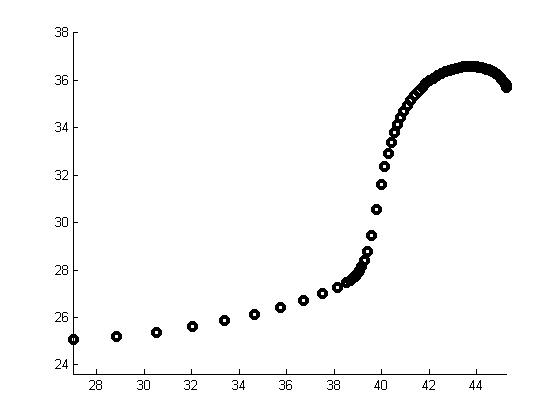
\includegraphics[width=0.2\textwidth] {PF-obstacle.png}
\end{center}
\caption{Potential Functions applied to robot and next position calculated using forward kinematic. Initial Pos: (25,25,0), Goal Position: (45,35), Obstacle Position: (42,28)}
\label{fig:PF_Path3}
\end{figure}
\vspace{-2 mm}
\section{Vision}
\vspace{-2 mm}
The primary aim of the Vision team was to integrate the previously independent system with the strategy and movement systems. A number of improvements were also added to the Vision module. A Canny edge detector was implemented in order to increase the quality of objects detected by object detection program. The previous implementation used the black spot at the end of the plate, with new improvements a second method was developed which calculates orientation using the plate which is dark green. Also, the learning platform has been improved using an SVM algorithm. We plan to test the learning platform for the later milestones.
The primary aim of the Vision team was to integrate the previously independent system with the strategy and movement systems. A number of improvements were also added to the Vision module. A Canny edge detector was also implemented in order to increase the quality of objects detected by object detection program. The previous implementation used the black spot at the end of the plate, with new improvements a second method is now used which calculates orientation using the plate with dark green. Also the learning platform has been improved using an SVM algorithm. We plan to test the learning platform for the later milestones.
\vspace{-2 mm}
\section{Simulator}
\vspace{-2 mm}
A good desgined simulator can play an important role in testing and integrating different algorithms. Strating from second milestone a simulator was desgined.
 
The developed simulator has two basic modes of operation. One accepts two types of commands which allow the robot the move forward or backward with a chosen speed and rotate in place. The other simulates the actual wheels of the robot and accepts two parameters which represent the speed of both wheels which allows it to move along a curved path and closely resembles the robot's real behavior, This is done by implementing Forward Kinematic of a differential Drive. The first one also supports collision detection for the pitch but the next step will be to generalize this for all objects on the field.

The simulator also outputs positions similar to what Vision module. This makes it easy to integrate different algorithms with vision module. 
\vspace{-2 mm}
\section{Conclusion}
\vspace{-2 mm}
While we made good headway into our goals for the second milestone, there were a number of problems which meant our results were not as good as we had hoped. The theory behind our work on planning and strategy is sound, and produces expected results when run on the simulator. However, hardware problems, predominantly with connecting the robot to a DICE machine running the Vision system via Bluetooth, meant that there was little time left before the milestone demonstration to test our system on the physical robot. The Vision and Movement systems were also not fully integrated at the time of the milestone, giving inaccurate and sometimes unpredictable results.

Durring the second milestone we learnt that a robust integrattion phase is required to make sure we can get what we develop seperately an in isolation of othe modules. The most import aspect of this is a good structure and connection of modules so if one fails other could continue working with backup plans. This can be done by developing loosly coupled modules and connected to each other using conventional approaches like Network TCP/IP or RPCs.

Over the next two weeks, much time will be spent on fully integrating the Vision and Movement systems. We will also put much more focus on testing and tuning the existing systems, as well as working on more advanced strategies. It is likely that the team will be reorganised again, to put more emphasis on working with the client/server code dealing with robot strategy and movement. 
\pagebreak
\bibliographystyle{IEEEtran}
\bibliography{bibliography}

\section{Appendix}
\subsection{Movement Testing} \label{mov:test}
Robot Movement Testing: Testing the robot’s ability to move forwards in a straight line.
Goal: Determine why robot does not move forward in a straight line.
Global conditions: Running program SpeedTest.njx, in which robot moves forwards, then backwards, then spins on the spot, at a motor speed of 700/1000. Single ball bearing rear wheel. Motors labelled A and B, wheels labelled A and B. Battery fully charged.
Testing ground: Second pitch.
\begin{figure}[htp]
\begin{center}
\leavevmode
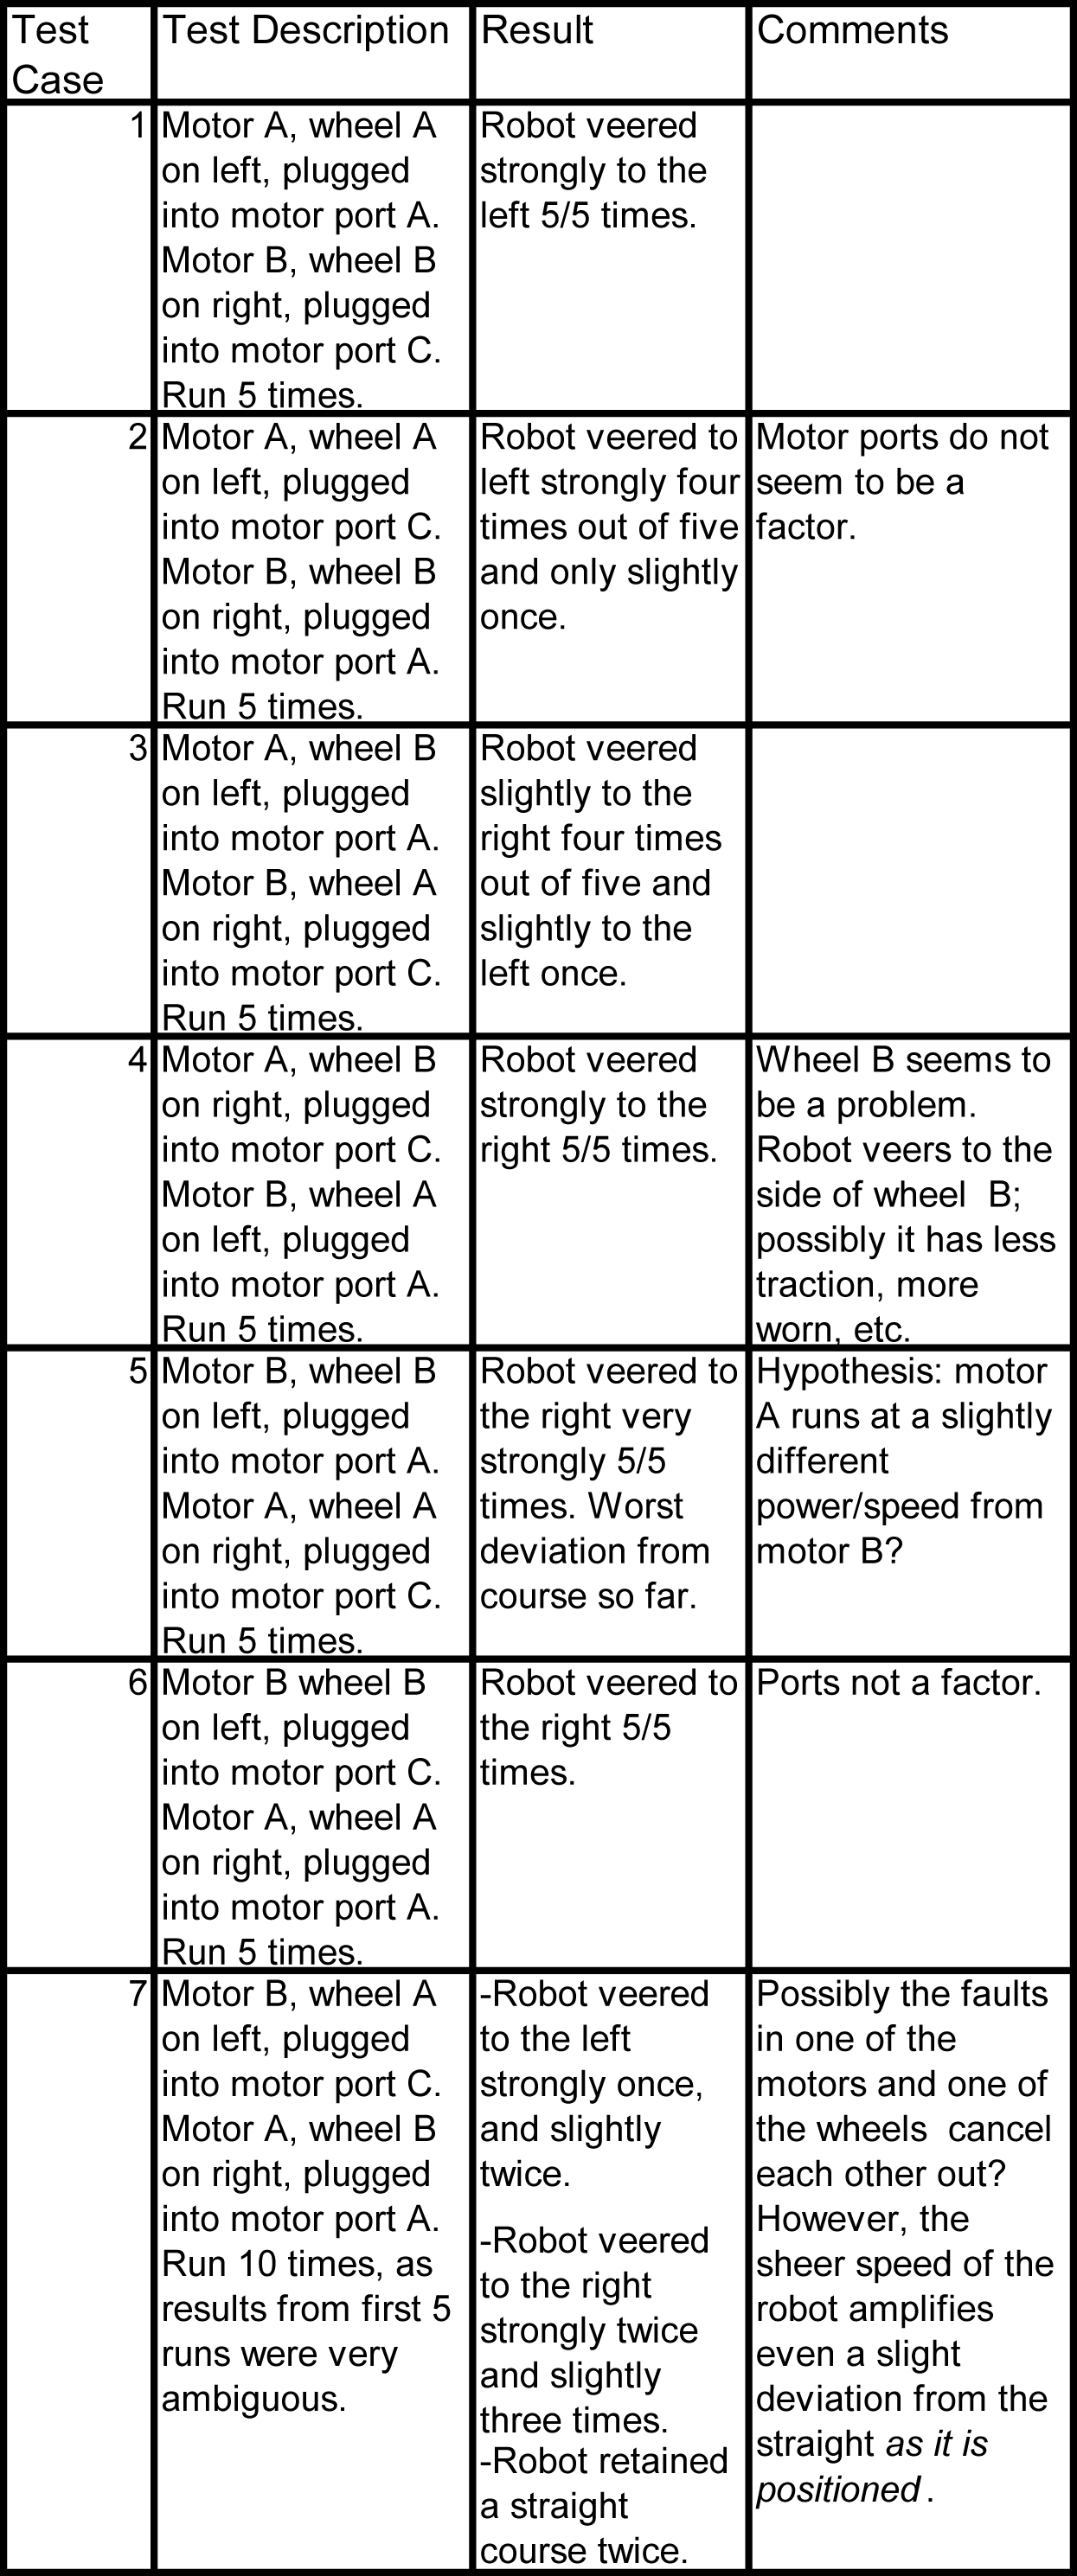
\includegraphics[width=0.3\textwidth] {tableOfTests.png}
\end{center}
\end{figure}

\subsection{Matlab figures} \label{fig:matlab}
\begin{figure}[htp]
\begin{center}
\leavevmode
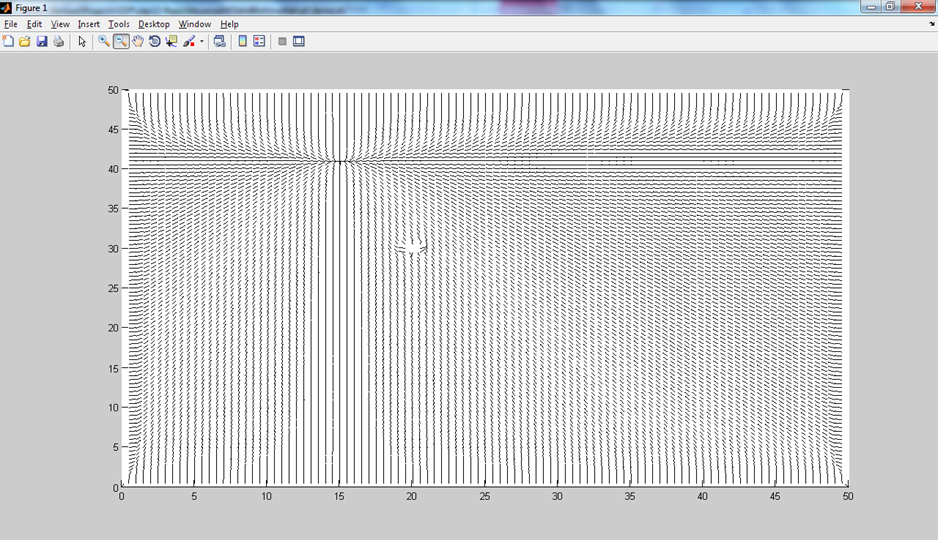
\includegraphics[width=0.4\textwidth] {PF.png}
\end{center}
\caption{Potential Functions in presence of obstacles. Vectors' sizes are normalized to 1, Goal Position: 15,45, Obstacle: (20,30)}
\label{fig:PF1}
\end{figure}

\begin{figure}[htp]
\begin{center}
\leavevmode
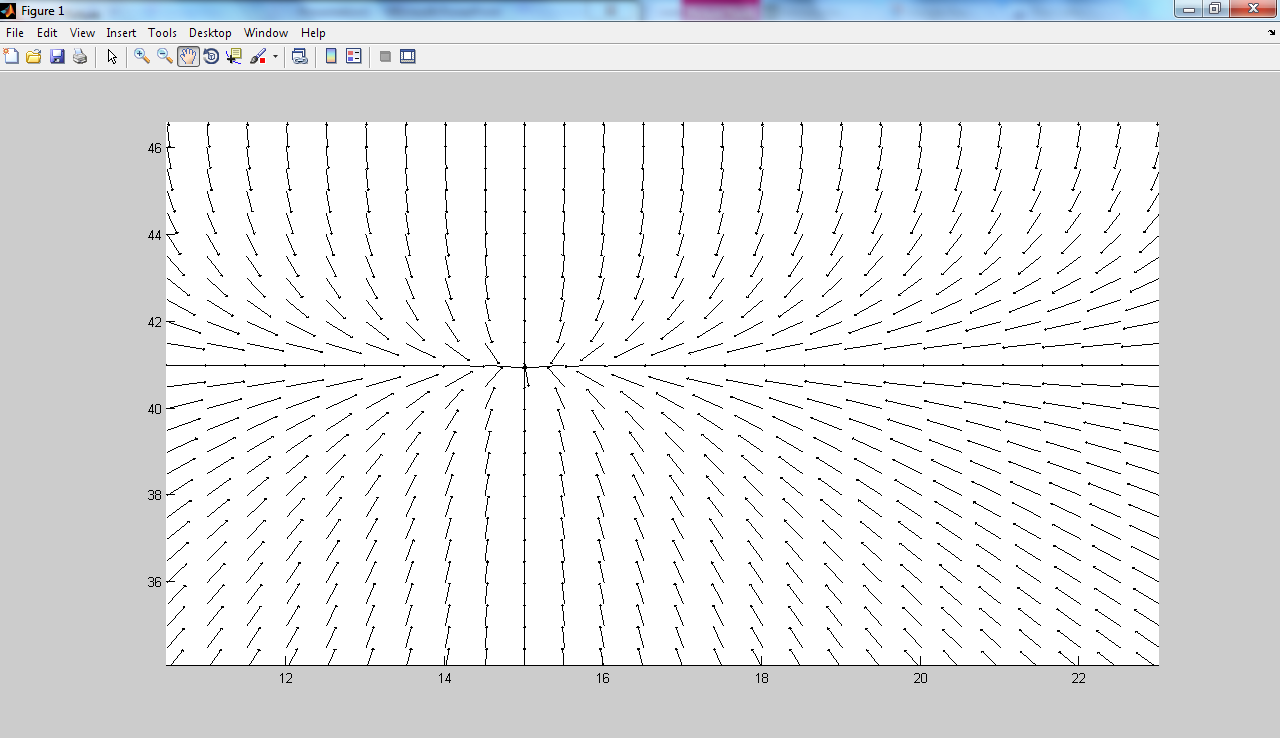
\includegraphics[width=0.4\textwidth] {PF-goal.png}
\end{center}
\caption{Potential Functions in presence of obstacles, zoomed in to Goal position. Vectors' sizes are normalized to 1, Goal Position: (15,45) , Obstacle: (20,30)}
\label{fig:PF2}
\end{figure}

\begin{figure}[htp]
\begin{center}
\leavevmode
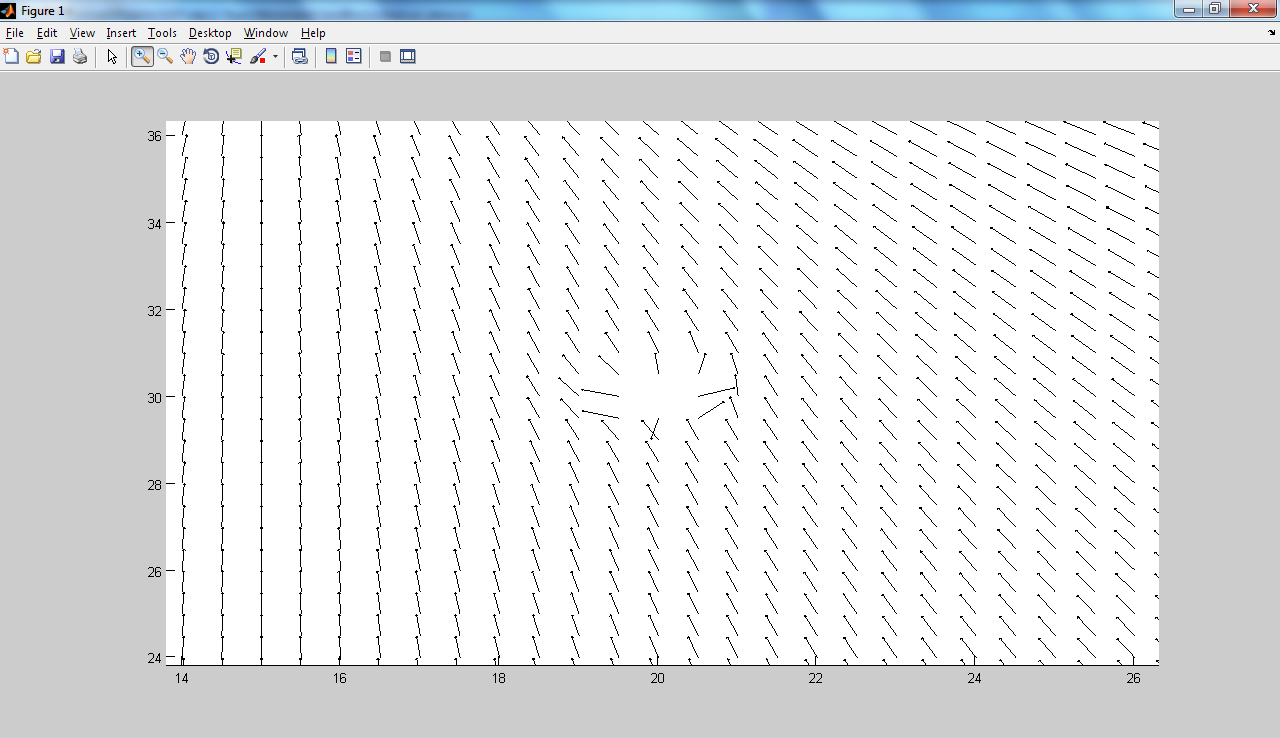
\includegraphics[width=0.4\textwidth] {PF-obs.png}
\end{center}
\caption{Potential Functions in presence of obstacles, zoomed in to Obstacle position. Vectors' sizes are normalized to 1, Goal Position: (15,45) , Obstacle: (20,30)}
\label{fig:PF3}
\end{figure}

\begin{figure}[htp]
\begin{center}
\leavevmode
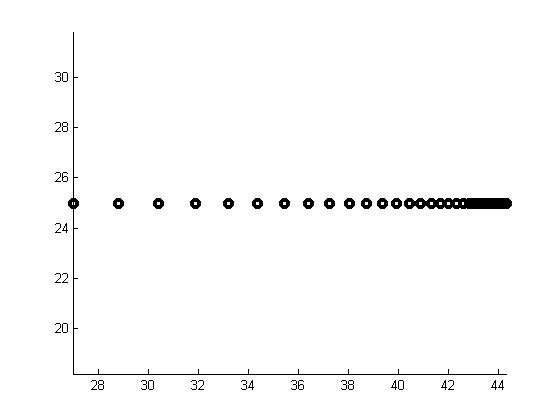
\includegraphics[width=0.4\textwidth] {PF-straight.png}
\end{center}
\caption{Potential Functions applied to robot and next position calculated using forward kinematic. Initial Pos: (25,25,0), Goal Position: (45,35)}
\label{fig:PF_Path1}
\end{figure}


\begin{figure}[htp]
\begin{center}
\leavevmode
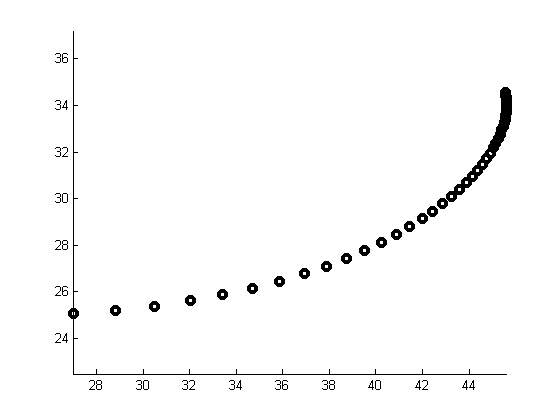
\includegraphics[width=0.4\textwidth] {PF-curve.png}
\end{center}
\caption{Potential Functions applied to robot and next position calculated using forward kinematic. Initial Pos: (25,25,0), Goal Position: (45,35)}
\label{fig:PF_Path2}
\end{figure}

\pagebreak

\begin{figure}[htp]
\begin{center}
\leavevmode

\includegraphics[width=0.4\textwidth] {logo.jpg}
\end{center}
\caption{Team Logo}
\label{fig:logo}
\end{figure}
\end{document}
